\section{Lecture 4: Zero sum games and infinite population games}
\newsection

\definition{Zero-sum game}{
    A two player game is said to be \textbf{zero-sum} if for any pure action profile $\bar{s}$,
    \[
    \pi_1(\bar{s})+\pi_2(\bar{s})=k
    \]
    for a constant $k$. WLOG we can assume $k=0$.
}
\begin{remark}
    This dates back to 1928 (von Neumann).
\end{remark}
\example{
    The following are examples of zero-sum games. These are ``strictly competitive'' settings.
    \begin{itemize}
        \item \hyperref[ex:ex:attackdefend]{Attacker/defender}
        \item Chess 
        \item Futures/options contracts in finance
        \item \hyperref[ex:cakecutting]{Cake-cutting}
        \item Worst case analysis in computer science.
    \end{itemize}
}
\begin{aexample}{Cake Cutting}{cakecutting}
    \begin{center}
        \begin{tabular}{|c|c c|} 
            \hline
            cutter\textbackslash chooser & Larger&Smaller \\ 
            \hline
            equal & (50,50) & (50,50)\\ 
            \hline
            unequal & (40,60)&(60,40)\\
            \hline
        \end{tabular}
    \end{center}
\end{aexample}

\example{
    Consider the zero-sum game with reward matrix \begin{center}
        \begin{tabular}{|c| c|} 
            \hline
             (1,-1) & (-1,1)\\ 
            \hline
             (-1,1)&(1,-1)\\
            \hline
        \end{tabular}
    \end{center}
    We can represent it as a single matrix\begin{center}
        \begin{tabular}{|c | c|} 
            \hline
             1 & -1\\ 
            \hline
             -1&1\\
            \hline
        \end{tabular}
    \end{center}
    Now the row player wants to maximize the value, and the column player wants to minimze the value. 
}
Now we suppose \[
    \bar{\sigma}_1=\begin{bmatrix}
        \sigma_{1,1}\\\sigma_{1,2}\\ \vdots \\ \sigma_{1,m}
    \end{bmatrix}
\] be a mixed strategy for player 1. Then $\bar\sigma_1^TA$ denotes the expected payoff of player 1 if player 2 chooses the corresponding column (pure strategy).
Therefore if $\bar\sigma_2$ denotes the mixed strategy of player 2, we have the expected value of player 1 is $\bar\sigma_1 ^T A\bar\sigma_2$.

\definition{Maxi-min/min-max strategies}{
    We define \[
    V_1^* \defeq \max_{\bar\sigma_1}\min_{\bar\sigma_2} \bar\sigma_1 ^T A\bar\sigma_2.
    \]
    This denotes the largest worst-case payoff for player 1.
    Similarly we define \[
        V_2^* \defeq \min_{\bar\sigma_2}  \max_{\bar\sigma_1}\bar\sigma_1 ^T A\bar\sigma_2.
        \]
}
\proposition{
    We have\[
    V_1^*\leq V_2^*.\]
}
\begin{proof}
     We have $V_1^*\leq \min_{\sigma_2} B_1(\bar\sigma_2) ^T A\bar\sigma_2=V_2^*.$
\end{proof}
\begin{atheorem}{Minimax}{minimax}
    For any $2$ player zero-sum game, \begin{itemize}
        \item $V_1^*=V_2^*$
        \item The set of Nash equilibria is $\{\bar\sigma_1^*,\bar\sigma_2^*\}$ for $\bar\sigma_1^*$ maximin and $\bar\sigma_2^*$ minimax. 
    \end{itemize}
\end{atheorem}
\begin{proof}
    Let $(\tilde{\sigma}_1,\tilde\sigma_2)$ be a Nash equilibrium. Then \[
    \tilde\sigma_1 = \arg \max_{\sigma_1} \sigma_1^T A\tilde\sigma_2
    \] 
     and \[
        \tilde\sigma_2 = \arg \min_{\sigma_2} \tilde\sigma_1^T A\sigma_2.
     \]
     So that \[
     V_2^* = \min_{\sigma_2} \max_{\sigma_1} \sigma_1^T A \sigma_2 \leq \max_{\sigma_1} \sigma_1^T A \tilde\sigma_2 \stackeq{nash}  \min_{\sigma_2} \tilde\sigma_1^T A \sigma_2  \leq \max_{\sigma_1}\min_{\sigma_2}\sigma_1^T A \sigma_2  = V_1^*.
     \]
     The proposition $V_1^*\leq V_2^*$ completes the proof.
\end{proof}
The compute this equilibrium, we find \begin{align*}
    \max_{\sigma_1}v,
\end{align*}
such that $[\sigma_1^TA]_j\geq v\forall j$, subject to $\sigma_{1,1}+\sigma_{1,2}+\cdots+\sigma_{1,m}=1$ and $\sigma_{1,j}\geq 0$. This is a linear program, so we can compute this in polynomial time. All hail Dinic and push relabel.

\definition{Infinite Population Games}{
    An \textbf{infinite population game} is a game where the set of players is infinite. 
}
\begin{aexample}{Infinite Population Game}{}
    Consider a game where the set of players is the continuum $[0,1]$, such that each player is infinitesimal. This is known as `non-atomic player with a mass of 1'. 
\end{aexample}
\begin{aexample}{Traffic Equilibrium}{}
    \begin{center}
        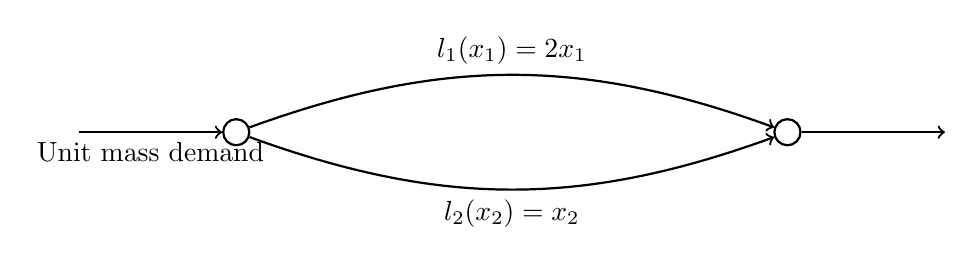
\begin{tikzpicture}
            \begin{scope}[every node/.style={circle,thick,draw}]
                \node (A) at (0,0) {};
                \node (B) at (7,0) {};
            \end{scope}
            \begin{scope}[every path/.style={->,thick}]
                \path [->] (-2,0) edge node[midway, below]{Unit mass demand}(A);
                \path [->] (A) edge [bend left=20] node[midway, above]{$l_1(x_1)=2x_1$}(B);
                \path [->] (A) edge [bend right=20] node[midway, below]{$l_2(x_2)=x_2$}(B);
                \path [->] (B) edge (9,0);
            \end{scope}
        \end{tikzpicture}
    \end{center}
    Suppose we have a unit mass of traffic going through two routes with $l_1$ or $l_2$ cost each. We find the nash equilibrium subject to $x_1+x_2=1$, $x_1,x_2\geq 0$. 
\end{aexample}
This is very intuitive. Relating $l_1(x_1)=l_2(x_2)$ gives $x_1=1/3,x_2=2/3$.
\begin{remark}
    This is also known as a \textbf{wardrop equilibrium}. The cost on all the paths used is the same. The cost on all the paths that are not used is greater than on the used paths.
\end{remark}

\begin{aexample}{Pigon}{pigon}
    Consider the following `traffic diagram'.
    \begin{center}
        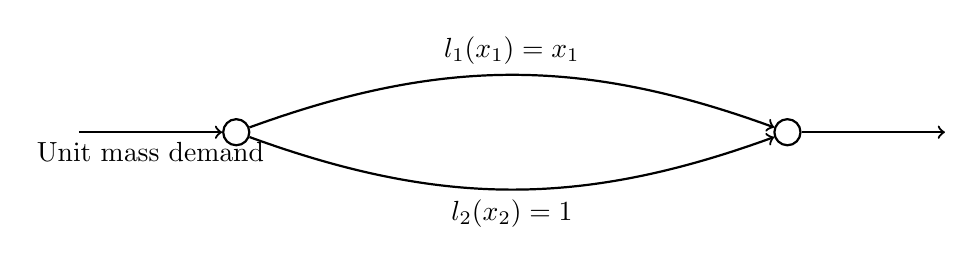
\begin{tikzpicture}
            
        \begin{scope}[every node/.style={circle,thick,draw}]
            \node (A) at (0,0) {};
            \node (B) at (7,0) {};
        \end{scope}
        \begin{scope}[every path/.style={->,thick}]
            \path [->] (-2,0) edge node[midway, below]{Unit mass demand}(A);
            \path [->] (A) edge [bend left=20] node[midway, above]{$l_1(x_1)=x_1$}(B);
            \path [->] (A) edge [bend right=20] node[midway, below]{$l_2(x_2)=1$}(B);
            \path [->] (B) edge (9,0);
        \end{scope}
        \end{tikzpicture}
    \end{center}
\end{aexample}
The wardrop equilibrium here is $x_1=1,x_2=0$. 
This is interesting, as we can consider the social cost, defined as the expected value of the cost for the players. In this case, everyone needs to pay a cost of $1$.

However, let us suppose that there is a planner who would like to minimize this total cost \[
\min_{x_1} x_1l(x_1)+x_2l(x_2) = \min x_1^2+(1-x_1).
\]
Completing the square gives a minimal cost when $x_1=1/2$ with a total cost of $3/4$. However, this is not a stable minima. There is an incentive to deviate from the assigned route.
    Let us define the price of anarchy \[
    P \defeq \frac{\textrm{cost with equilibrium}}{\textrm{cost with planner}}.
    \]
$P=1$ is the best outcome. But in this case we have a price of $1/(3/4) = 4/3$.
Consider the following diagram.
\begin{center}
    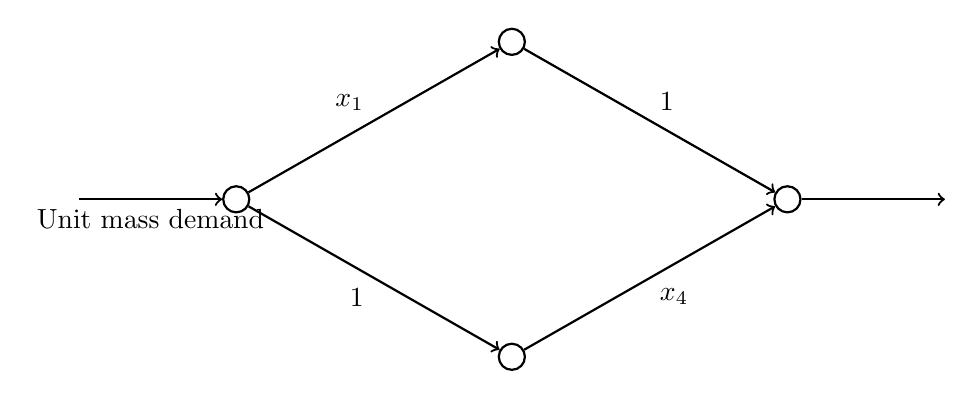
\begin{tikzpicture}
        
    \begin{scope}[every node/.style={circle,thick,draw}]
        \node (A) at (0,0) {};
        \node (B) at (7,0) {};
        \node (C) at (3.5,2){};
        \node (D) at (3.5,-2){};
    \end{scope}
    \begin{scope}[every path/.style={->,thick}]
        \path [->] (-2,0) edge node[midway, below]{Unit mass demand}(A);
        \path [->] (A) edge node[midway, above left] {$x_1$}(C);
        \path [->] (A) edge node[midway, below left] {$1$}(D);
        \path [->] (C) edge node[midway, above right] {$1$}(B);
        \path [->] (D) edge node[midway, below right] {$x_4$}(B);
        \path [->] (B) edge (9,0);
    \end{scope}
    \end{tikzpicture}\end{center}

Now, the equilibrium is when $x_1=x_4=1/2$, with a total social cost of $3/2$.
    Suppose we now create a new road.

    \begin{center}
        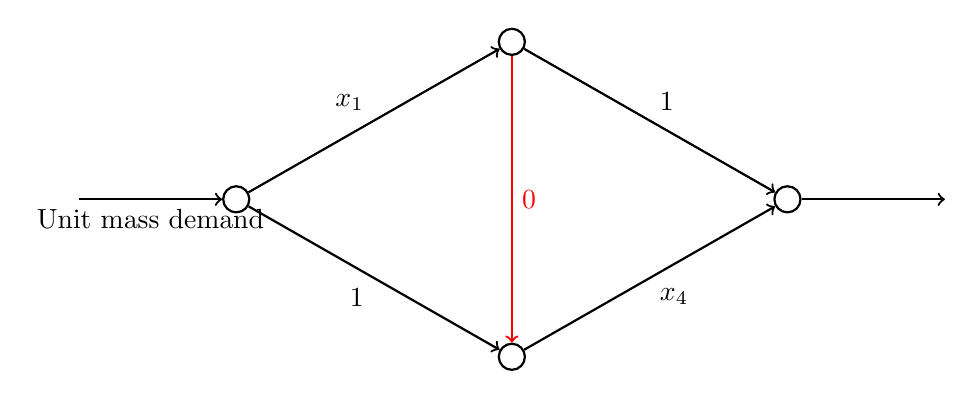
\begin{tikzpicture}
            
        \begin{scope}[every node/.style={circle,thick,draw}]
            \node (A) at (0,0) {};
            \node (B) at (7,0) {};
            \node (C) at (3.5,2){};
            \node (D) at (3.5,-2){};
        \end{scope}
        \begin{scope}[every path/.style={->,thick}]
            \path [->] (-2,0) edge node[midway, below]{Unit mass demand}(A);
            \path [->] (A) edge node[midway, above left] {$x_1$}(C);
            \path [->] (A) edge node[midway, below left] {$1$}(D);
            \path [->] (C) edge node[midway, above right] {$1$}(B);
            \path [->] (D) edge node[midway, below right] {$x_4$}(B);
            \path[red](C)edge node[midway, right]{$0$}(D); 
            \path [->] (B) edge (9,0);
        \end{scope}
        \end{tikzpicture}\end{center}

Now, the best road is to go up then through the red edge. This means the new equilibrium now is $x_1=x_4=1$ with a total social cost of $2$. This is known as \textbf{Braess's paradox}, where adding more resources to the system causes the social cost to increase.

\subsection*{Existence of Wardrop Equilibria}.
We want to determine when wardrop equilibria exist in the following graph.

\begin{center}
    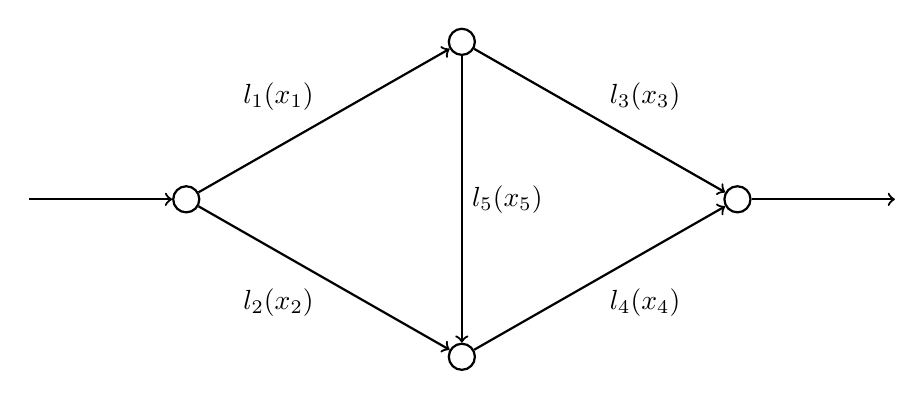
\begin{tikzpicture}
        
    \begin{scope}[every node/.style={circle,thick,draw}]
        \node (A) at (0,0) {};
        \node (B) at (7,0) {};
        \node (C) at (3.5,2){};
        \node (D) at (3.5,-2){};
    \end{scope}
    \begin{scope}[every path/.style={->,thick}]
        \path [->] (-2,0) edge (A);
        \path [->] (A) edge node[midway, above left] {$l_1(x_1)$}(C);
        \path [->] (A) edge node[midway, below left] {$l_2(x_2)$}(D);
        \path [->] (C) edge node[midway, above right] {$l_3(x_3)$}(B);
        \path [->] (D) edge node[midway, below right] {$l_4(x_4)$}(B);
        \path(C)edge node[midway, right]{$l_5(x_5)$}(D); 
        \path [->] (B) edge (9,0);
    \end{scope}
\end{tikzpicture}\end{center}
\begin{atheorem}{}{}
    Assume that each $l_i(x_i)$ is non-negative, non-decreasing, and differentiable. Then a unique Wardrop Equilibrium exists.
\end{atheorem}
\begin{proof}[Sketch of proof]
    Let $P$ be the set of all paths from the source to the destination.
    Let $x_p$ be the number of users on path $i$, and $E$ be the set of edges. We now have an optimization \[
        \min_{\{x_p:p\in P\} } \sum_{i\in E} \int_{0}^{\textrm{total traffic on $i$}} l_i(z) dz
    \]
    subject to $\sum_{p\in P} x_p=1, x_p\geq 0 \forall p\in P$.

    We claim that this optimization problem has a unique solution, and this solution is the Wardrop equilibrium. The argument boils down to showing that the function is convex,thus has a unique minimum. 

    Let $\lambda$ be a Lagrange Multiplier for the condition $\sum_{p\in P} x_p=1$. Then the first order optimality shows that \[
    \sum_{\textrm{edges in path $p$}} l_i(\sum_{\textrm{paths $p$ using $i$}}x_p)\geq \lambda
    \]
    with equality when $\sum {x_p}>0$.
\end{proof}
